% Created by tikzDevice version 0.12.3.1 on 2023-02-19 11:33:20
% !TEX encoding = UTF-8 Unicode
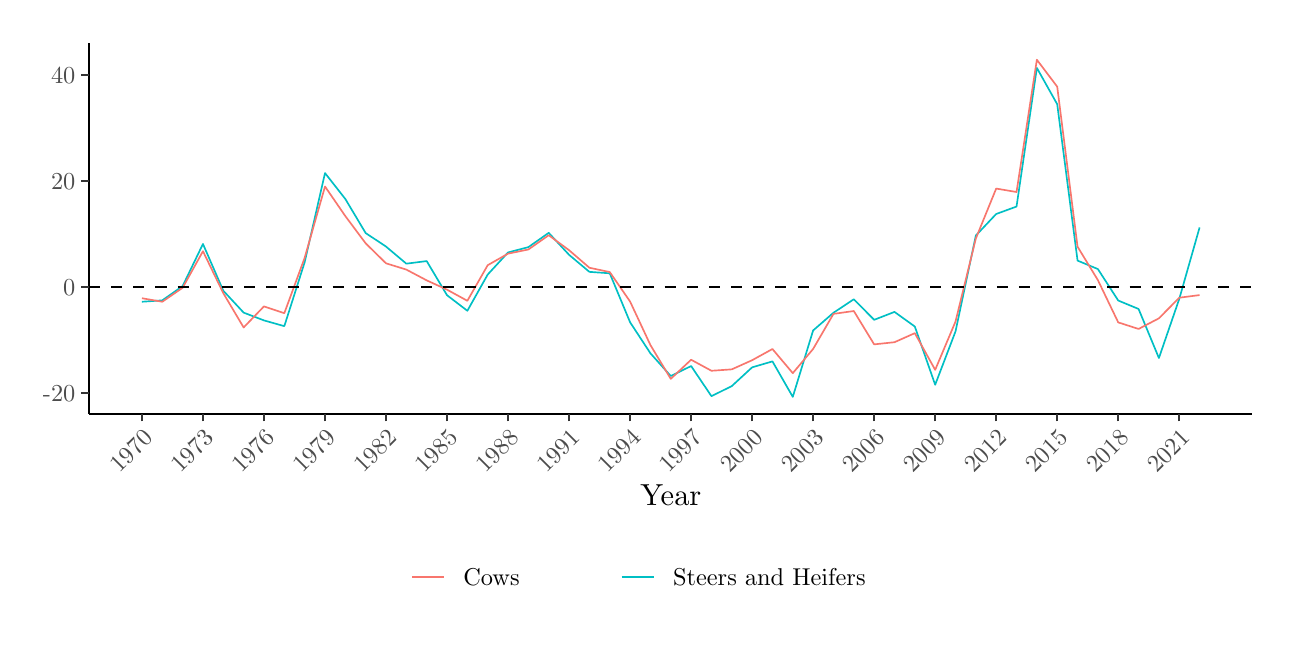
\begin{tikzpicture}[x=1pt,y=1pt]
\definecolor{fillColor}{RGB}{255,255,255}
\path[use as bounding box,fill=fillColor,fill opacity=0.00] (0,0) rectangle (448.07,216.81);
\begin{scope}
\path[clip] (  0.00,  0.00) rectangle (448.07,216.81);
\definecolor{drawColor}{RGB}{255,255,255}
\definecolor{fillColor}{RGB}{255,255,255}

\path[draw=drawColor,line width= 0.6pt,line join=round,line cap=round,fill=fillColor] (  0.00,  0.00) rectangle (448.07,216.81);
\end{scope}
\begin{scope}
\path[clip] ( 22.18, 77.31) rectangle (442.57,211.31);
\definecolor{fillColor}{RGB}{255,255,255}

\path[fill=fillColor] ( 22.18, 77.31) rectangle (442.57,211.31);
\definecolor{drawColor}{RGB}{0,191,196}

\path[draw=drawColor,line width= 0.6pt,line join=round] ( 41.29,117.77) --
	( 48.64,118.27) --
	( 55.99,123.43) --
	( 63.34,138.65) --
	( 70.69,121.76) --
	( 78.04,113.84) --
	( 85.39,111.03) --
	( 92.74,108.95) --
	(100.09,132.06) --
	(107.44,164.27) --
	(114.78,154.91) --
	(122.13,142.60) --
	(129.48,137.71) --
	(136.83,131.53) --
	(144.18,132.47) --
	(151.53,120.13) --
	(158.88,114.51) --
	(166.23,127.60) --
	(173.58,135.59) --
	(180.93,137.51) --
	(188.28,142.67) --
	(195.63,134.73) --
	(202.98,128.57) --
	(210.33,128.05) --
	(217.68,110.36) --
	(225.03, 99.14) --
	(232.38, 90.93) --
	(239.73, 94.54) --
	(247.08, 83.65) --
	(254.43, 87.30) --
	(261.78, 94.07) --
	(269.12, 96.22) --
	(276.47, 83.40) --
	(283.82,107.40) --
	(291.17,113.79) --
	(298.52,118.68) --
	(305.87,111.24) --
	(313.22,114.10) --
	(320.57,108.82) --
	(327.92, 87.78) --
	(335.27,107.04) --
	(342.62,141.70) --
	(349.97,149.48) --
	(357.32,152.17) --
	(364.67,202.26) --
	(372.02,189.15) --
	(379.37,132.64) --
	(386.72,129.58) --
	(394.07,118.21) --
	(401.42,115.16) --
	(408.77, 97.43) --
	(416.12,118.79) --
	(423.47,144.62);
\definecolor{drawColor}{RGB}{248,118,109}

\path[draw=drawColor,line width= 0.6pt,line join=round] ( 41.29,119.04) --
	( 48.64,117.77) --
	( 55.99,122.82) --
	( 63.34,136.03) --
	( 70.69,120.87) --
	( 78.04,108.48) --
	( 85.39,116.10) --
	( 92.74,113.64) --
	(100.09,133.65) --
	(107.44,159.41) --
	(114.78,148.73) --
	(122.13,138.88) --
	(129.48,131.66) --
	(136.83,129.39) --
	(144.18,125.50) --
	(151.53,122.14) --
	(158.88,118.12) --
	(166.23,130.98) --
	(173.58,135.15) --
	(180.93,136.66) --
	(188.28,141.81) --
	(195.63,136.40) --
	(202.98,130.06) --
	(210.33,128.50) --
	(217.68,117.85) --
	(225.03,102.12) --
	(232.38, 89.91) --
	(239.73, 96.82) --
	(247.08, 92.83) --
	(254.43, 93.34) --
	(261.78, 96.65) --
	(269.12,100.69) --
	(276.47, 91.97) --
	(283.82,100.72) --
	(291.17,113.39) --
	(298.52,114.42) --
	(305.87,102.37) --
	(313.22,103.15) --
	(320.57,106.42) --
	(327.92, 93.16) --
	(335.27,110.60) --
	(342.62,140.63) --
	(349.97,158.67) --
	(357.32,157.42) --
	(364.67,205.22) --
	(372.02,195.48) --
	(379.37,137.66) --
	(386.72,125.58) --
	(394.07,110.31) --
	(401.42,107.94) --
	(408.77,111.78) --
	(416.12,119.23) --
	(423.47,120.18);
\definecolor{drawColor}{RGB}{0,0,0}

\path[draw=drawColor,line width= 0.6pt,dash pattern=on 4pt off 4pt ,line join=round] ( 22.18,122.99) -- (442.57,122.99);
\end{scope}
\begin{scope}
\path[clip] (  0.00,  0.00) rectangle (448.07,216.81);
\definecolor{drawColor}{RGB}{0,0,0}

\path[draw=drawColor,line width= 0.6pt,line join=round] ( 22.18, 77.31) --
	( 22.18,211.31);
\end{scope}
\begin{scope}
\path[clip] (  0.00,  0.00) rectangle (448.07,216.81);
\definecolor{drawColor}{gray}{0.30}

\node[text=drawColor,anchor=base east,inner sep=0pt, outer sep=0pt, scale=  0.88] at ( 17.23, 81.65) {-20};

\node[text=drawColor,anchor=base east,inner sep=0pt, outer sep=0pt, scale=  0.88] at ( 17.23,119.96) {0};

\node[text=drawColor,anchor=base east,inner sep=0pt, outer sep=0pt, scale=  0.88] at ( 17.23,158.26) {20};

\node[text=drawColor,anchor=base east,inner sep=0pt, outer sep=0pt, scale=  0.88] at ( 17.23,196.57) {40};
\end{scope}
\begin{scope}
\path[clip] (  0.00,  0.00) rectangle (448.07,216.81);
\definecolor{drawColor}{gray}{0.20}

\path[draw=drawColor,line width= 0.6pt,line join=round] ( 19.43, 84.68) --
	( 22.18, 84.68);

\path[draw=drawColor,line width= 0.6pt,line join=round] ( 19.43,122.99) --
	( 22.18,122.99);

\path[draw=drawColor,line width= 0.6pt,line join=round] ( 19.43,161.29) --
	( 22.18,161.29);

\path[draw=drawColor,line width= 0.6pt,line join=round] ( 19.43,199.60) --
	( 22.18,199.60);
\end{scope}
\begin{scope}
\path[clip] (  0.00,  0.00) rectangle (448.07,216.81);
\definecolor{drawColor}{RGB}{0,0,0}

\path[draw=drawColor,line width= 0.6pt,line join=round] ( 22.18, 77.31) --
	(442.57, 77.31);
\end{scope}
\begin{scope}
\path[clip] (  0.00,  0.00) rectangle (448.07,216.81);
\definecolor{drawColor}{gray}{0.20}

\path[draw=drawColor,line width= 0.6pt,line join=round] ( 41.29, 74.56) --
	( 41.29, 77.31);

\path[draw=drawColor,line width= 0.6pt,line join=round] ( 63.34, 74.56) --
	( 63.34, 77.31);

\path[draw=drawColor,line width= 0.6pt,line join=round] ( 85.39, 74.56) --
	( 85.39, 77.31);

\path[draw=drawColor,line width= 0.6pt,line join=round] (107.44, 74.56) --
	(107.44, 77.31);

\path[draw=drawColor,line width= 0.6pt,line join=round] (129.48, 74.56) --
	(129.48, 77.31);

\path[draw=drawColor,line width= 0.6pt,line join=round] (151.53, 74.56) --
	(151.53, 77.31);

\path[draw=drawColor,line width= 0.6pt,line join=round] (173.58, 74.56) --
	(173.58, 77.31);

\path[draw=drawColor,line width= 0.6pt,line join=round] (195.63, 74.56) --
	(195.63, 77.31);

\path[draw=drawColor,line width= 0.6pt,line join=round] (217.68, 74.56) --
	(217.68, 77.31);

\path[draw=drawColor,line width= 0.6pt,line join=round] (239.73, 74.56) --
	(239.73, 77.31);

\path[draw=drawColor,line width= 0.6pt,line join=round] (261.78, 74.56) --
	(261.78, 77.31);

\path[draw=drawColor,line width= 0.6pt,line join=round] (283.82, 74.56) --
	(283.82, 77.31);

\path[draw=drawColor,line width= 0.6pt,line join=round] (305.87, 74.56) --
	(305.87, 77.31);

\path[draw=drawColor,line width= 0.6pt,line join=round] (327.92, 74.56) --
	(327.92, 77.31);

\path[draw=drawColor,line width= 0.6pt,line join=round] (349.97, 74.56) --
	(349.97, 77.31);

\path[draw=drawColor,line width= 0.6pt,line join=round] (372.02, 74.56) --
	(372.02, 77.31);

\path[draw=drawColor,line width= 0.6pt,line join=round] (394.07, 74.56) --
	(394.07, 77.31);

\path[draw=drawColor,line width= 0.6pt,line join=round] (416.12, 74.56) --
	(416.12, 77.31);
\end{scope}
\begin{scope}
\path[clip] (  0.00,  0.00) rectangle (448.07,216.81);
\definecolor{drawColor}{gray}{0.30}

\node[text=drawColor,rotate= 45.00,anchor=base east,inner sep=0pt, outer sep=0pt, scale=  0.88] at ( 45.57, 68.07) {1970};

\node[text=drawColor,rotate= 45.00,anchor=base east,inner sep=0pt, outer sep=0pt, scale=  0.88] at ( 67.62, 68.07) {1973};

\node[text=drawColor,rotate= 45.00,anchor=base east,inner sep=0pt, outer sep=0pt, scale=  0.88] at ( 89.67, 68.07) {1976};

\node[text=drawColor,rotate= 45.00,anchor=base east,inner sep=0pt, outer sep=0pt, scale=  0.88] at (111.72, 68.07) {1979};

\node[text=drawColor,rotate= 45.00,anchor=base east,inner sep=0pt, outer sep=0pt, scale=  0.88] at (133.77, 68.07) {1982};

\node[text=drawColor,rotate= 45.00,anchor=base east,inner sep=0pt, outer sep=0pt, scale=  0.88] at (155.82, 68.07) {1985};

\node[text=drawColor,rotate= 45.00,anchor=base east,inner sep=0pt, outer sep=0pt, scale=  0.88] at (177.87, 68.07) {1988};

\node[text=drawColor,rotate= 45.00,anchor=base east,inner sep=0pt, outer sep=0pt, scale=  0.88] at (199.92, 68.07) {1991};

\node[text=drawColor,rotate= 45.00,anchor=base east,inner sep=0pt, outer sep=0pt, scale=  0.88] at (221.96, 68.07) {1994};

\node[text=drawColor,rotate= 45.00,anchor=base east,inner sep=0pt, outer sep=0pt, scale=  0.88] at (244.01, 68.07) {1997};

\node[text=drawColor,rotate= 45.00,anchor=base east,inner sep=0pt, outer sep=0pt, scale=  0.88] at (266.06, 68.07) {2000};

\node[text=drawColor,rotate= 45.00,anchor=base east,inner sep=0pt, outer sep=0pt, scale=  0.88] at (288.11, 68.07) {2003};

\node[text=drawColor,rotate= 45.00,anchor=base east,inner sep=0pt, outer sep=0pt, scale=  0.88] at (310.16, 68.07) {2006};

\node[text=drawColor,rotate= 45.00,anchor=base east,inner sep=0pt, outer sep=0pt, scale=  0.88] at (332.21, 68.07) {2009};

\node[text=drawColor,rotate= 45.00,anchor=base east,inner sep=0pt, outer sep=0pt, scale=  0.88] at (354.26, 68.07) {2012};

\node[text=drawColor,rotate= 45.00,anchor=base east,inner sep=0pt, outer sep=0pt, scale=  0.88] at (376.30, 68.07) {2015};

\node[text=drawColor,rotate= 45.00,anchor=base east,inner sep=0pt, outer sep=0pt, scale=  0.88] at (398.35, 68.07) {2018};

\node[text=drawColor,rotate= 45.00,anchor=base east,inner sep=0pt, outer sep=0pt, scale=  0.88] at (420.40, 68.07) {2021};
\end{scope}
\begin{scope}
\path[clip] (  0.00,  0.00) rectangle (448.07,216.81);
\definecolor{drawColor}{RGB}{0,0,0}

\node[text=drawColor,anchor=base,inner sep=0pt, outer sep=0pt, scale=  1.10] at (232.38, 44.09) {Year};
\end{scope}
\begin{scope}
\path[clip] (  0.00,  0.00) rectangle (448.07,216.81);
\definecolor{fillColor}{RGB}{255,255,255}

\path[fill=fillColor] (126.48,  5.50) rectangle (338.27, 30.95);
\end{scope}
\begin{scope}
\path[clip] (  0.00,  0.00) rectangle (448.07,216.81);
\definecolor{drawColor}{RGB}{248,118,109}

\path[draw=drawColor,line width= 0.6pt,line join=round] (138.93, 18.23) -- (150.49, 18.23);
\end{scope}
\begin{scope}
\path[clip] (  0.00,  0.00) rectangle (448.07,216.81);
\definecolor{drawColor}{RGB}{248,118,109}

\path[draw=drawColor,line width= 0.6pt,line join=round] (138.93, 18.23) -- (150.49, 18.23);
\end{scope}
\begin{scope}
\path[clip] (  0.00,  0.00) rectangle (448.07,216.81);
\definecolor{drawColor}{RGB}{0,191,196}

\path[draw=drawColor,line width= 0.6pt,line join=round] (214.71, 18.23) -- (226.28, 18.23);
\end{scope}
\begin{scope}
\path[clip] (  0.00,  0.00) rectangle (448.07,216.81);
\definecolor{drawColor}{RGB}{0,191,196}

\path[draw=drawColor,line width= 0.6pt,line join=round] (214.71, 18.23) -- (226.28, 18.23);
\end{scope}
\begin{scope}
\path[clip] (  0.00,  0.00) rectangle (448.07,216.81);
\definecolor{drawColor}{RGB}{0,0,0}

\node[text=drawColor,anchor=base west,inner sep=0pt, outer sep=0pt, scale=  0.88] at (157.43, 15.20) {Cows};
\end{scope}
\begin{scope}
\path[clip] (  0.00,  0.00) rectangle (448.07,216.81);
\definecolor{drawColor}{RGB}{0,0,0}

\node[text=drawColor,anchor=base west,inner sep=0pt, outer sep=0pt, scale=  0.88] at (233.22, 15.20) {Steers and Heifers};
\end{scope}
\end{tikzpicture}
